% Phoenix AI - Enterprise Documentation Q&A Assistant
% Compile with: pdflatex phoenix_ai.tex   (or upload to Overleaf)
\documentclass[aspectratio=169,11pt]{beamer}

\usetheme{Madrid}
\usecolortheme{default}
\usepackage[utf8]{inputenc}
\usepackage[T1]{fontenc}
\usepackage{tikz}
\usetikzlibrary{positioning,arrows.meta,shapes.geometric,fit,backgrounds}
\usepackage{booktabs}
\usepackage{array}
% left-aligned paragraph column (no stretched spacing or hyphenation)
\newcolumntype{L}[1]{>{\raggedright\arraybackslash}p{#1}}

% ---------- colours ----------
\definecolor{phoenix}{RGB}{31,78,121}
\definecolor{flame}{RGB}{230,92,0}
\definecolor{softblue}{RGB}{220,230,241}
\definecolor{softorange}{RGB}{253,235,220}
\definecolor{softgreen}{RGB}{226,240,217}
\setbeamercolor{structure}{fg=phoenix}
\setbeamercolor{title}{fg=white,bg=phoenix}
\setbeamercolor{frametitle}{fg=white,bg=phoenix}
\setbeamercolor{block title}{fg=white,bg=phoenix}
\setbeamercolor{block body}{bg=softblue}
\setbeamercolor{block title alerted}{fg=white,bg=flame}
\setbeamercolor{block body alerted}{bg=softorange}
\setbeamercolor{block title example}{fg=white,bg=green!45!black}
\setbeamercolor{block body example}{bg=softgreen}
\setbeamertemplate{navigation symbols}{}
\setbeamertemplate{itemize items}[circle]

\newcommand{\code}[1]{\texttt{\small #1}}

% Title page order: title -> hackathon (subtitle) -> team name -> members (author)
\title[Enterprise Docs Q\&A Assistant]{Enterprise Documentation Q\&A Assistant}
\subtitle{\textbf{HCLTech Hackathon}}
\author[Phoenix AI]{{\large\textbf{Team Phoenix AI}}\\[0.8em]
  MANASVI \quad $\cdot$ \quad SAIM TANVEER \quad $\cdot$ \quad SWETHA}
\institute[HCLTech Hackathon]{}
\date{}

\begin{document}

% =====================================================================
% 1. TITLE
% =====================================================================
\begin{frame}[plain]
  \titlepage
  \vspace{-1.2em}
  \begin{center}
    \small\color{gray} Retrieval-Augmented Generation \;$\cdot$\; Role-based access \;$\cdot$\;
    Conflict-aware answers \;$\cdot$\; Measured evaluation
  \end{center}
\end{frame}

% =====================================================================
% 2. ARCHITECTURE
% =====================================================================
\begin{frame}{System Architecture}
  \centering
  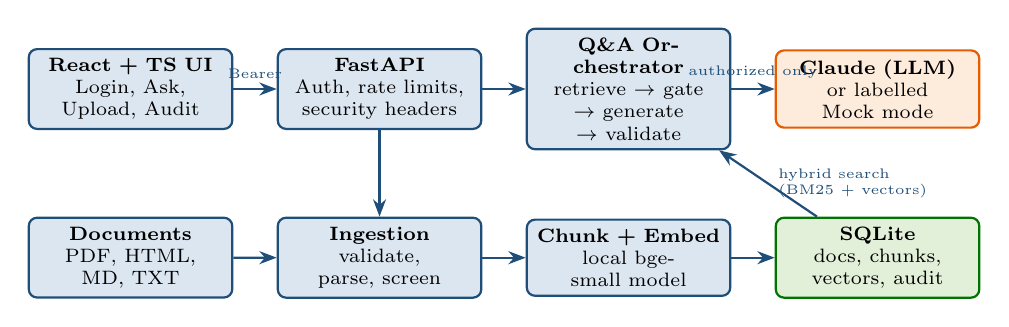
\begin{tikzpicture}[
      node distance=0.45cm and 0.55cm,
      box/.style={draw=phoenix, thick, rounded corners=3pt, fill=softblue, align=center,
                  font=\scriptsize, minimum height=0.95cm, text width=2.35cm},
      ext/.style={box, fill=softorange, draw=flame},
      store/.style={box, fill=softgreen, draw=green!45!black},
      arr/.style={-{Stealth[length=2.2mm]}, thick, phoenix}]
    % row 1: user flow
    \node[box] (ui) {\textbf{React + TS UI}\\Login, Ask, Upload, Audit};
    \node[box, right=of ui] (api) {\textbf{FastAPI}\\Auth, rate limits, security headers};
    \node[box, right=of api] (qa) {\textbf{Q\&A Orchestrator}\\retrieve $\rightarrow$ gate $\rightarrow$ generate $\rightarrow$ validate};
    \node[ext, right=of qa] (llm) {\textbf{Claude (LLM)}\\or labelled\\Mock mode};
    % row 2: ingestion
    \node[box, below=1.1cm of api] (ing) {\textbf{Ingestion}\\validate, parse, screen};
    \node[box, right=of ing] (chunk) {\textbf{Chunk + Embed}\\local bge-small model};
    \node[store, right=of chunk] (db) {\textbf{SQLite}\\docs, chunks, vectors, audit};
    \node[box, below=1.1cm of ui] (docs) {\textbf{Documents}\\PDF, HTML, MD, TXT};
    % arrows
    \draw[arr] (ui) -- node[above, font=\tiny]{Bearer} (api);
    \draw[arr] (api) -- (qa);
    \draw[arr] (qa) -- node[above, font=\tiny]{authorized only} (llm);
    \draw[arr] (docs) -- (ing);
    \draw[arr] (api) -- (ing);
    \draw[arr] (ing) -- (chunk);
    \draw[arr] (chunk) -- (db);
    \draw[arr] (db) -- node[right, font=\tiny, align=left]{hybrid search\\(BM25 + vectors)} (qa);
  \end{tikzpicture}

  \vspace{0.5em}
  \begin{columns}[T]
    \column{0.32\textwidth}
      \begin{block}{Get documents in}\scriptsize Upload $\rightarrow$ checks $\rightarrow$ passages with permissions\end{block}
    \column{0.32\textwidth}
      \begin{block}{Get answers out}\scriptsize Authorized search $\rightarrow$ cited, validated answer\end{block}
    \column{0.32\textwidth}
      \begin{block}{Keep it safe}\scriptsize Roles, audit log, injection \& secret screening\end{block}
  \end{columns}
\end{frame}

% =====================================================================
% COMPONENT 1 - GETTING DOCUMENTS IN  (Presenter: MANASVI)
% =====================================================================
\begin{frame}{Component 1: How a Document Becomes Searchable \hfill{\normalsize\color{white}(1/2)}}
  \centering
  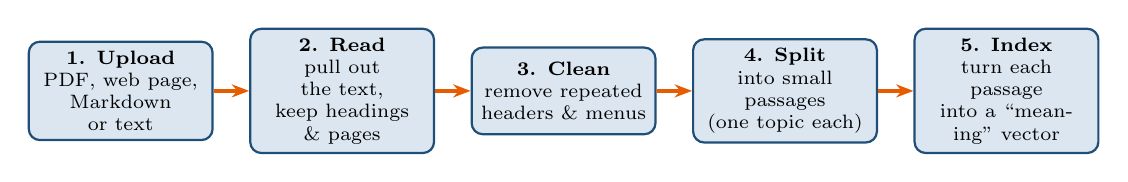
\begin{tikzpicture}[
      stage/.style={draw=phoenix, thick, rounded corners=4pt, fill=softblue, align=center,
                   font=\scriptsize, text width=2.1cm, minimum height=1.1cm},
      arr/.style={-{Stealth[length=2.2mm]}, very thick, flame}]
    \node[stage] (a) {\textbf{1. Upload}\\PDF, web page,\\Markdown or text};
    \node[stage, right=0.45cm of a] (b) {\textbf{2. Read}\\pull out the text,\\keep headings \& pages};
    \node[stage, right=0.45cm of b] (c) {\textbf{3. Clean}\\remove repeated\\headers \& menus};
    \node[stage, right=0.45cm of c] (d) {\textbf{4. Split}\\into small passages\\(one topic each)};
    \node[stage, right=0.45cm of d] (e) {\textbf{5. Index}\\turn each passage\\into a ``meaning'' vector};
    \draw[arr] (a) -- (b); \draw[arr] (b) -- (c); \draw[arr] (c) -- (d); \draw[arr] (d) -- (e);
  \end{tikzpicture}

  \vspace{0.6em}
  \begin{columns}[T]
    \column{0.5\textwidth}
      \textbf{Why we split documents into passages}
      \begin{itemize}\small
        \item A question needs one paragraph, not a 50-page manual
        \item Each passage remembers its \textbf{document, section and page} --- so we can cite it later
        \item A passage never mixes two sections or two product versions
        \item Step-by-step instructions are kept together
      \end{itemize}
    \column{0.47\textwidth}
      \begin{exampleblock}{Example}\small
        \textbf{Account\_Access\_Guide.pdf} becomes 5 passages, e.g.\\[0.2em]
        \textit{``Password Reset'' --- page 1}\\
        ``Reset links expire after 30 minutes.''
      \end{exampleblock}
      \begin{block}{Nothing is guessed}\small
        Version and date are saved only if the document states them.
      \end{block}
  \end{columns}
\end{frame}

\begin{frame}{Component 1: Keeping Bad Files Out \hfill{\normalsize\color{white}(2/2)}}
  \begin{columns}[T]
    \column{0.55\textwidth}
      \textbf{Every upload is checked before it is used}\\[0.4em]
      \footnotesize
      \renewcommand{\arraystretch}{1.25}
      \begin{tabular}{@{}L{3.5cm}L{3.9cm}@{}}
        \toprule
        \textbf{If someone uploads\ldots} & \textbf{What happens} \\
        \midrule
        a program renamed to \code{.pdf} & \textbf{rejected} -- content is checked, not the name \\
        a scanned (image-only) PDF & \textbf{rejected} with a clear message (no OCR) \\
        an empty or duplicate file & \textbf{rejected} \\
        a file over 10 MB, or too slow to read & \textbf{rejected} / reading stopped \\
        a file containing a password or key & \textbf{quarantined} -- never searchable \\
        text like ``ignore previous instructions'' & \textbf{flagged} -- waits for admin approval \\
        \bottomrule
      \end{tabular}
    \column{0.42\textwidth}
      \begin{alertblock}{Only trusted content is searchable}\small
        Employees cannot publish.\\
        HR and Sales uploads wait until an \textbf{Admin approves} them.
      \end{alertblock}
      \begin{block}{Tamper check}\small
        Each file gets a digital fingerprint (hash) when approved.
        If the stored file is changed later, downloading it is blocked.
      \end{block}
  \end{columns}
\end{frame}

% =====================================================================
% COMPONENT 2 - RETRIEVAL & ANSWERS  (Presenter: SAIM TANVEER)
% =====================================================================
\begin{frame}{Component 2: Hybrid Retrieval \hfill{\normalsize\color{white}(1/2)}}
  \begin{columns}[T]
    \column{0.5\textwidth}
      \textbf{Permissions first, then search}
      \begin{enumerate}\small
        \item Keep only passages the user may read
        \item \textbf{BM25 keywords} --- exact codes like \code{E104}
        \item \textbf{Vector similarity} --- paraphrases
        \item Reciprocal-rank fusion + error-code and version boosts
        \item Evidence gate: nothing close enough $\Rightarrow$ ``not found'', never a guess
      \end{enumerate}
    \column{0.47\textwidth}
      \begin{exampleblock}{Example}\small
        ``\textit{I forgot my login password}''\\
        $\rightarrow$ \textbf{Account Access Guide $>$ Password Reset}, page 1
      \end{exampleblock}
      \begin{block}{Developer debug view}\small
        Shows every authorized passage retrieved with its dense, BM25 and fused scores.\\[0.2em]
        Scores are ranking signals --- \textbf{no fake confidence percentages}.
      \end{block}
  \end{columns}
\end{frame}

\begin{frame}{Component 2: Grounded Answers, Citations \& Conflicts \hfill{\normalsize\color{white}(2/2)}}
  \begin{columns}[T]
    \column{0.5\textwidth}
      \textbf{Answers you can verify}
      \begin{itemize}\small
        \item Claude answers \textbf{only} from retrieved evidence, as structured JSON
        \item Every citation must point to a passage retrieved for this question
        \item Statements with numbers missing from the source are removed
        \item Citations: title, section, PDF page, verbatim excerpt --- permission re-checked on click
      \end{itemize}
      \vspace{0.3em}
      {\scriptsize\textbf{5 states:} answered $\cdot$ partially answered $\cdot$ clarification needed $\cdot$ conflicting evidence $\cdot$ not found}
    \column{0.47\textwidth}
      \begin{alertblock}{Conflict handling}\small
        Manual v2: \textbf{20 MB} \;vs\; Release Notes v3: \textbf{50 MB}\\
        $\rightarrow$ both cited, asks \textit{``Which product version are you using?''}\\[0.4em]
        Same version, different values $\rightarrow$ \textbf{conflicting evidence}.\\
        No source is silently chosen.
      \end{alertblock}
  \end{columns}
\end{frame}

% =====================================================================
% COMPONENT 3 - SECURITY & PROOF  (Presenter: SWETHA)
% =====================================================================
\begin{frame}{Component 3: Who Can See What \hfill{\normalsize\color{white}(1/2)}}
  \begin{columns}[T]
    \column{0.5\textwidth}
      \textbf{Every user has a role}\\[0.3em]
      \small
      \begin{tabular}{@{}ll@{}}
        \toprule
        \textbf{Role} & \textbf{Can read} \\
        \midrule
        Employee & general documents \\
        Sales & general documents \\
        HR & general + \textbf{HR-only} documents \\
        Admin & everything; approves \& manages \\
        \bottomrule
      \end{tabular}

      \vspace{0.5em}
      \textbf{How it is enforced}
      \begin{itemize}\small
        \item Checked on the \textbf{server} every time --- the browser cannot fake a role
        \item Restricted documents are removed \textbf{before} searching, so the AI never sees them
        \item Opening a citation or download is checked again
      \end{itemize}
    \column{0.47\textwidth}
      \begin{exampleblock}{Same question, two users}\small
        \textit{``What is the salary band for L3?''}\\[0.3em]
        \textbf{Sales} $\rightarrow$ ``I could not find that information in the documents available to you.''\\[0.2em]
        \textbf{HR} $\rightarrow$ answered, with a citation to the HR policy
      \end{exampleblock}
      \begin{block}{Everything is logged}\small
        An audit log records who did what and whether it was allowed --- visible to Admins only.
      \end{block}
  \end{columns}
\end{frame}

\begin{frame}{Component 3: How We Know It Works \hfill{\normalsize\color{white}(2/2)}}
  \begin{columns}[T]
    \column{0.45\textwidth}
      \textbf{We tried to break it}
      \begin{itemize}\small
        \item \textbf{54} automatic backend tests + \textbf{5} UI tests --- all pass
        \item \textbf{30} live attack checks: guessing IDs, faking roles, bad files, hidden instructions --- \textbf{30/30 pass}
        \item \textbf{0} leaks of HR data in any test
      \end{itemize}
      \textbf{We measured answer quality}
      \begin{itemize}\small
        \item 42 test questions with known correct answers
        \item 20 of them kept hidden until the end
      \end{itemize}
    \column{0.52\textwidth}
      \small
      \begin{tabular}{@{}lcc@{}}
        \toprule
        \textbf{Result} & \textbf{Practice} & \textbf{Hidden} \\
        \midrule
        Right passage in top 3 & 100\% & 100\% \\
        Correct answer type & 95\% & 55\%$^{*}$ \\
        Conflicts handled & 2/2 & 2/2 \\
        Restricted data leaked & 0 & 0 \\
        \bottomrule
      \end{tabular}\\[0.4em]
      \begin{alertblock}{Honest result}\scriptsize
        $^{*}$Search is perfect; the drop comes from the simple offline answer writer (mock mode) misjudging
        paraphrased questions. 65\% after fixes. Live Claude results need an API key.
      \end{alertblock}
  \end{columns}
\end{frame}

% =====================================================================
% THANK YOU
% =====================================================================
\begin{frame}[plain]
  \centering
  \vspace{2.2em}
  {\Huge\bfseries\color{phoenix} Thank You!}\\[1.2em]
  {\Large Questions?}\\[2em]
  {\large\textbf{Team Phoenix AI}}\\[0.4em]
  MANASVI \quad $\cdot$ \quad SAIM TANVEER \quad $\cdot$ \quad SWETHA\\[1.5em]
  {\small\color{gray} Answers only from documents you may read \;$\cdot$\; every claim cited \;$\cdot$\;
  honest ``not found''}
\end{frame}

\end{document}
